\documentclass[11pt,a4paper]{article}

% ── Paquetes ─────────────────────────────────────────────────────────────────
\usepackage[utf8]{inputenc}
\usepackage[T1]{fontenc}
\usepackage[spanish,es-noshorthands,es-tabla]{babel}
\usepackage{lmodern}
\usepackage[margin=2.3cm]{geometry}
\usepackage{graphicx}
\usepackage{booktabs}
\usepackage{tabularx}
\usepackage{amsmath}
\usepackage{xcolor}
\usepackage{caption}
\usepackage{subcaption}
\usepackage{listings}
\usepackage{tikz}
\usetikzlibrary{positioning,arrows.meta}
\usepackage{enumitem}
\usepackage[hidelinks]{hyperref}

\graphicspath{{../figuras/}}
\definecolor{principal}{HTML}{2A6F97}
\definecolor{secundario}{HTML}{E07A5F}
\definecolor{gris}{HTML}{8D99AE}
\setlist{itemsep=2pt, topsep=4pt}
\captionsetup{font=small, labelfont=bf}

\lstset{
  basicstyle=\ttfamily\footnotesize,
  keywordstyle=\color{principal}\bfseries,
  commentstyle=\color{gris},
  language=SQL, morekeywords={LEFT},
  frame=single, rulecolor=\color{gris!60},
  columns=fullflexible, keepspaces=true, showstringspaces=false,
  aboveskip=6pt, belowskip=6pt
}

\newcommand{\gw}[1]{#1~GW}

\begin{document}

% ── Portada ──────────────────────────────────────────────────────────────────
\begin{titlepage}
\centering
{\scshape Universidad de Buenos Aires · Facultad de Ciencias Económicas\par}
{\small Tecnicatura Universitaria en Gestión y Análisis de Datos en Organizaciones\par}
\vspace{0.4cm}\rule{\textwidth}{0.6pt}\vspace{2.2cm}

{\Huge\bfseries ¿Cuánta electricidad se come la IA?\par}
\vspace{0.5cm}
{\Large Data centers de inteligencia artificial: potencia, energía,\\ localización y un escenario para Argentina\par}
\vspace{1.8cm}

{\large Trabajo práctico modelo\par}
\vspace{0.3cm}
{Laboratorio de Métodos Cuantitativos Aplicados a la Gestión\par}
\vspace{0.6cm}
{\large Juan Ignacio Da Torre \quad · \quad Joaquín Romano\par}

\vfill
\begin{tabular}{rl}
\textbf{Código:} & \url{https://github.com/Datso653/datacenters-ia} \\
\textbf{Notebook:} & \texttt{notebooks/analisis\_datacenters.ipynb} \\
\textbf{Fecha:} & septiembre de 2026 \\
\end{tabular}
\vspace{1cm}
\end{titlepage}

% ── Resumen ──────────────────────────────────────────────────────────────────
\begin{abstract}
\noindent
Este trabajo cuantifica la demanda eléctrica de los grandes data centers de inteligencia artificial y la dimensiona frente al sistema eléctrico argentino. Se combinan cuatro fuentes públicas —Epoch AI, la EIA de Estados Unidos y Our World in Data— unidas por nombre, estado y país, y se valida cada unión con consultas SQL equivalentes. Sobre la serie de potencia instalada se aplican derivadas (velocidad de instalación) e integrales (energía consumida). Los 69 data centers operativos suman \gw{12,9} y consumen del orden de 118~TWh al año, el 73\,\% de la demanda eléctrica argentina; con las obras en curso, la cifra se duplicaría respecto de ese total. En Estados Unidos se ubican en estados con electricidad industrial más barata pero con un 62\,\% de generación fósil. Un proyecto de 500~MW en Argentina demandaría el 2,8\,\% de la electricidad del país y emitiría 1,6~Mt de CO$_2$ anuales con la red promedio.
\end{abstract}

% ═════════════════════════════════════════════════════════════════════════════
\section{Introducción}

La inteligencia artificial suele discutirse como un fenómeno de software, pero su insumo crítico es físico: la \textbf{electricidad}. Entrenar y operar modelos requiere instalaciones con decenas de miles de chips que consumen, cada una, tanta potencia como una ciudad mediana. En octubre de 2025, OpenAI y la firma Sur Energy firmaron una carta de intención para construir en la Patagonia un data center de hasta 500~MW (\emph{Stargate Argentina}), con una inversión anunciada de USD~25.000 millones bajo el Régimen de Incentivo para Grandes Inversiones (RIGI). A septiembre de 2026 el proyecto no tiene sitio ni obra confirmados. El contexto financiero es de euforia: Anthropic y OpenAI presentaron en junio de 2026 pedidos confidenciales de salida a bolsa, con valuaciones privadas de USD~965.000 y 852.000 millones respectivamente \cite{cnbcanthropic,tcopenai}.

Dimensionar un proyecto así exige números: cuánto consume, cómo se compara con la red del país, cuánto emitiría y cuánto costaría. La pregunta que guía el trabajo es:

\begin{quote}
\itshape ¿Cuánta electricidad demandan los grandes data centers de IA, a qué ritmo crece esa demanda y qué implicaría —en energía, emisiones y costo— instalar uno de 500~MW en Argentina?
\end{quote}

% ═════════════════════════════════════════════════════════════════════════════
\section{Datos y metodología}

\subsection{Fuentes}

\begin{table}[h]
\centering\small
\begin{tabularx}{\textwidth}{@{}l X l@{}}
\toprule
\textbf{Fuente} & \textbf{Contenido} & \textbf{Unidad} \\
\midrule
Epoch AI — \emph{AI Data Centers} (sep-2026) & 86 data centers: potencia IT, cómputo (H100 equivalentes), dueño, dirección; 499 hitos de obra & data center \\
Epoch AI — \emph{GPU Clusters} (mar-2026) & 482 clusters en 36 países & cluster \\
EIA (Estados Unidos) & Precio medio de la electricidad y generación por fuente, 2024 & estado \\
Our World in Data (Ember, IEA) & Demanda eléctrica (TWh), intensidad de carbono (gCO$_2$/kWh) y \% consumido por data centers & país / región \\
\bottomrule
\end{tabularx}
\caption{Fuentes utilizadas. Todas son públicas; las de Epoch y OWID tienen licencia CC-BY 4.0.}
\label{tab:fuentes}
\end{table}

La base de data centers es, en la práctica, una fotografía de Estados Unidos: 75 de los 86 registros están en ese país. Diecisiete tienen potencia nula porque están en construcción. La exploración reveló un dato metodológico central: \textbf{el costo de capital por MW es idéntico en todos los registros} (37,9 millones de USD por MW, con desvío nulo). Epoch no mide el costo de cada instalación sino que lo estima con un coeficiente fijo, por lo que no es posible estimar una función de costos; esos coeficientes se usan únicamente como parámetros de escenario.

\subsection{Transformaciones}

\begin{enumerate}
\item \textbf{Limpieza de etiquetas de confianza} (\texttt{"Google \#confident"} $\to$ \texttt{"Google"}), para que cada dueño sea una única categoría.
\item \textbf{Construcción de la clave \texttt{estado}} a partir de la dirección, mediante expresiones regulares; en 10 casos sin dirección utilizable se asignó a partir del nombre del proyecto o sus fuentes.
\item \textbf{Filtro de operativos} (potencia $>0$): 69 de 86.
\item \textbf{Grilla mensual de potencia}: cada data center arrastra su último valor conocido (\emph{forward fill}) para poder sumar hitos informados en fechas distintas.
\item \textbf{Normalización de nombres de país} entre Epoch y OWID.
\end{enumerate}

\subsection{Cruce de las bases}

Ninguna fuente responde la pregunta por sí sola. La Figura~\ref{fig:cruces} resume las uniones: todas son \texttt{LEFT JOIN}, porque la tabla de la izquierda es la unidad de análisis y no debe perder registros aunque falte el dato de la derecha.

\begin{figure}[h]
\centering
\begin{tikzpicture}[
  tabla/.style={draw=principal, fill=principal!8, rounded corners=3pt, minimum width=3.2cm, minimum height=0.85cm, font=\small\bfseries, align=center},
  fuente/.style={draw=gris, fill=gris!10, rounded corners=3pt, minimum width=3.2cm, minimum height=0.85cm, font=\small, align=center},
  flecha/.style={-{Stealth[length=2.5mm]}, thick, color=principal!80},
  clave/.style={font=\scriptsize\ttfamily, fill=white, inner sep=1.5pt}
]
\node[tabla] (dc) {data\_centers\\[-2pt]{\scriptsize\normalfont Epoch · 86}};
\node[fuente, right=2.6cm of dc, yshift=1.1cm] (tl) {timelines\\[-2pt]{\scriptsize Epoch · 499 hitos}};
\node[fuente, right=2.6cm of dc] (pr) {precios 2024\\[-2pt]{\scriptsize EIA · 52}};
\node[fuente, right=2.6cm of dc, yshift=-1.1cm] (mx) {mix eléctrico 2024\\[-2pt]{\scriptsize EIA · 52}};

\node[tabla, below=2.2cm of dc] (gc) {gpu\_clusters\\[-2pt]{\scriptsize\normalfont Epoch · 482}};
\node[fuente, right=2.6cm of gc, yshift=0.55cm] (ci) {intensidad CO$_2$\\[-2pt]{\scriptsize OWID · 220 países}};
\node[fuente, right=2.6cm of gc, yshift=-0.55cm] (de) {demanda eléctrica\\[-2pt]{\scriptsize OWID}};

\draw[flecha] (dc.east) -- node[clave, above, sloped] {nombre} (tl.west);
\draw[flecha] (dc.east) -- node[clave, above] {estado} (pr.west);
\draw[flecha] (dc.east) -- node[clave, below, sloped] {estado} (mx.west);
\draw[flecha] (gc.east) -- node[clave, above, sloped] {pais} (ci.west);
\draw[flecha] (gc.east) -- node[clave, below, sloped] {pais} (de.west);
\end{tikzpicture}
\caption{Mapa de cruces. En azul, las tablas protagonistas; en gris, las que aportan columnas. Sobre las flechas, la clave de unión.}
\label{fig:cruces}
\end{figure}

Antes de cada unión se diagnosticó la cobertura de claves (Tabla~\ref{tab:cobertura}). El caso ilustrativo es el de los países: sin normalizar, solo coincidían 34 de 36, y los dos ausentes eran \emph{United States of America} (el país con más potencia) y \emph{Philippines (the)}. Un \emph{merge} no advierte este error: simplemente devuelve valores nulos.

\begin{table}[h]
\centering\small
\begin{tabular}{@{}lccc@{}}
\toprule
\textbf{Cruce} & \textbf{Clave} & \textbf{Claves que coinciden} & \textbf{Cobertura} \\
\midrule
data centers $\to$ línea de tiempo & nombre & 86 / 86 & 100\,\% \\
data centers EE.UU. $\to$ EIA & estado & 29 / 29 & 100\,\% \\
clusters $\to$ OWID (sin normalizar) & país & 34 / 36 & 94,4\,\% \\
clusters $\to$ OWID (normalizado) & país & 36 / 36 & 100\,\% \\
\bottomrule
\end{tabular}
\caption{Cobertura de claves por cruce. Además, 16 clusters no informan país (en su mayoría sistemas chinos anonimizados por la fuente).}
\label{tab:cobertura}
\end{table}

Siguiendo la unidad de \emph{SQL y manejo de tablas} de la materia, las tablas se cargaron en una base \texttt{sqlite3} en memoria y cada unión se reescribió como consulta. Por ejemplo, el cruce por estado:

\noindent\begin{minipage}{\linewidth}
\begin{lstlisting}
SELECT d.estado, COUNT(*) AS data_centers, SUM(d.mw_it) AS mw_it,
       p.precio_industrial, m.pct_fosil
FROM data_centers d
LEFT JOIN precios_2024 p ON d.estado = p.estado
LEFT JOIN mix_2024     m ON d.estado = m.estado
WHERE d.pais = 'United States' AND d.operativo = 1
GROUP BY d.estado
ORDER BY mw_it DESC
\end{lstlisting}
\end{minipage}

El resultado de la consulta coincide exactamente con el obtenido en pandas (\texttt{merge} + \texttt{groupby}), lo que funciona como control cruzado de la implementación.

\subsection{Derivadas e integrales}

Sea $P(t)$ la potencia IT instalada (MW). Se calculan:
\begin{align*}
P'(t) &\approx \frac{P(t+1)-P(t-1)}{2\,\Delta t} && \text{(velocidad de instalación, GW por año)} \\
E &= \int P(t)\cdot \mathrm{PUE}\cdot u \; dt && \text{(energía consumida, TWh)}
\end{align*}
La derivada se obtiene por diferencias centradas (\texttt{numpy.gradient}) y la integral por la regla del trapecio sobre la grilla mensual. El PUE (potencia total sobre potencia IT, que incorpora refrigeración y pérdidas) se fijó en 1,30, la mediana de la base. El factor de uso $u$ no se observa: se supuso $u=0{,}8$ y se sensibilizó. Las emisiones resultan de multiplicar la energía por la intensidad de carbono de la red: $\text{Mt CO}_2 = \text{TWh} \times \text{gCO}_2/\text{kWh} / 1000$.

Herramientas: Python (pandas, NumPy, Matplotlib, sqlite3) en Google Colab. El análisis es reproducible desde cero: datos crudos en \texttt{data/raw/}, módulos en \texttt{src/} y notebook ejecutado en \texttt{notebooks/} (\texttt{pip install -r requirements.txt} y \texttt{python -m src.descarga}).

% ═════════════════════════════════════════════════════════════════════════════
\section{Resultados}

\subsection{Crecimiento: una curva explosiva}

La potencia de los data centers relevados pasó de \gw{0,4} en enero de 2024 a \gw{1,9} en enero de 2025 y a \gw{12,9} en septiembre de 2026 (Figura~\ref{fig:potencia}). Si se completan las obras en curso, alcanzaría \gw{35,5} hacia 2029. La derivada muestra una aceleración sostenida: 3,0~GW por año en 2025, 7,1 en 2026 y cerca de 10 en 2027--2028; luego cae porque la base solo contiene proyectos ya anunciados. La energía acumulada es, en consecuencia, convexa: entre enero y septiembre de 2026 estos data centers consumieron cerca de 57~TWh, casi cuatro veces la demanda anual de Uruguay.

\begin{figure}[h]
\centering
\begin{subfigure}{0.49\textwidth}
  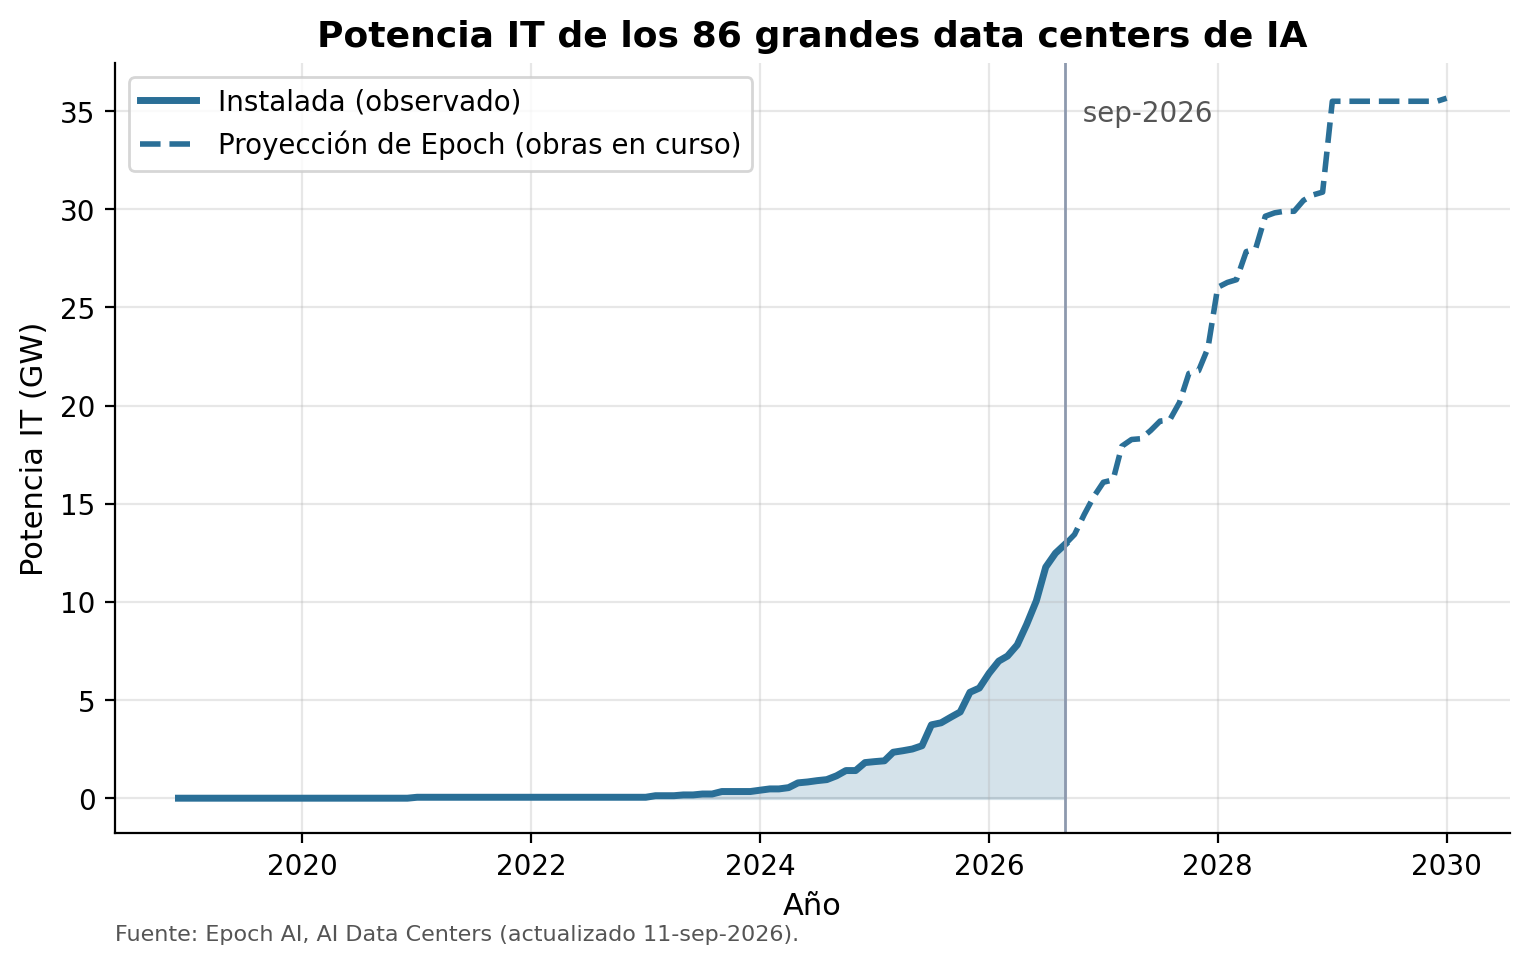
\includegraphics[width=\linewidth]{01_potencia_en_el_tiempo.png}
  \caption{Potencia IT agregada.}
\end{subfigure}\hfill
\begin{subfigure}{0.49\textwidth}
  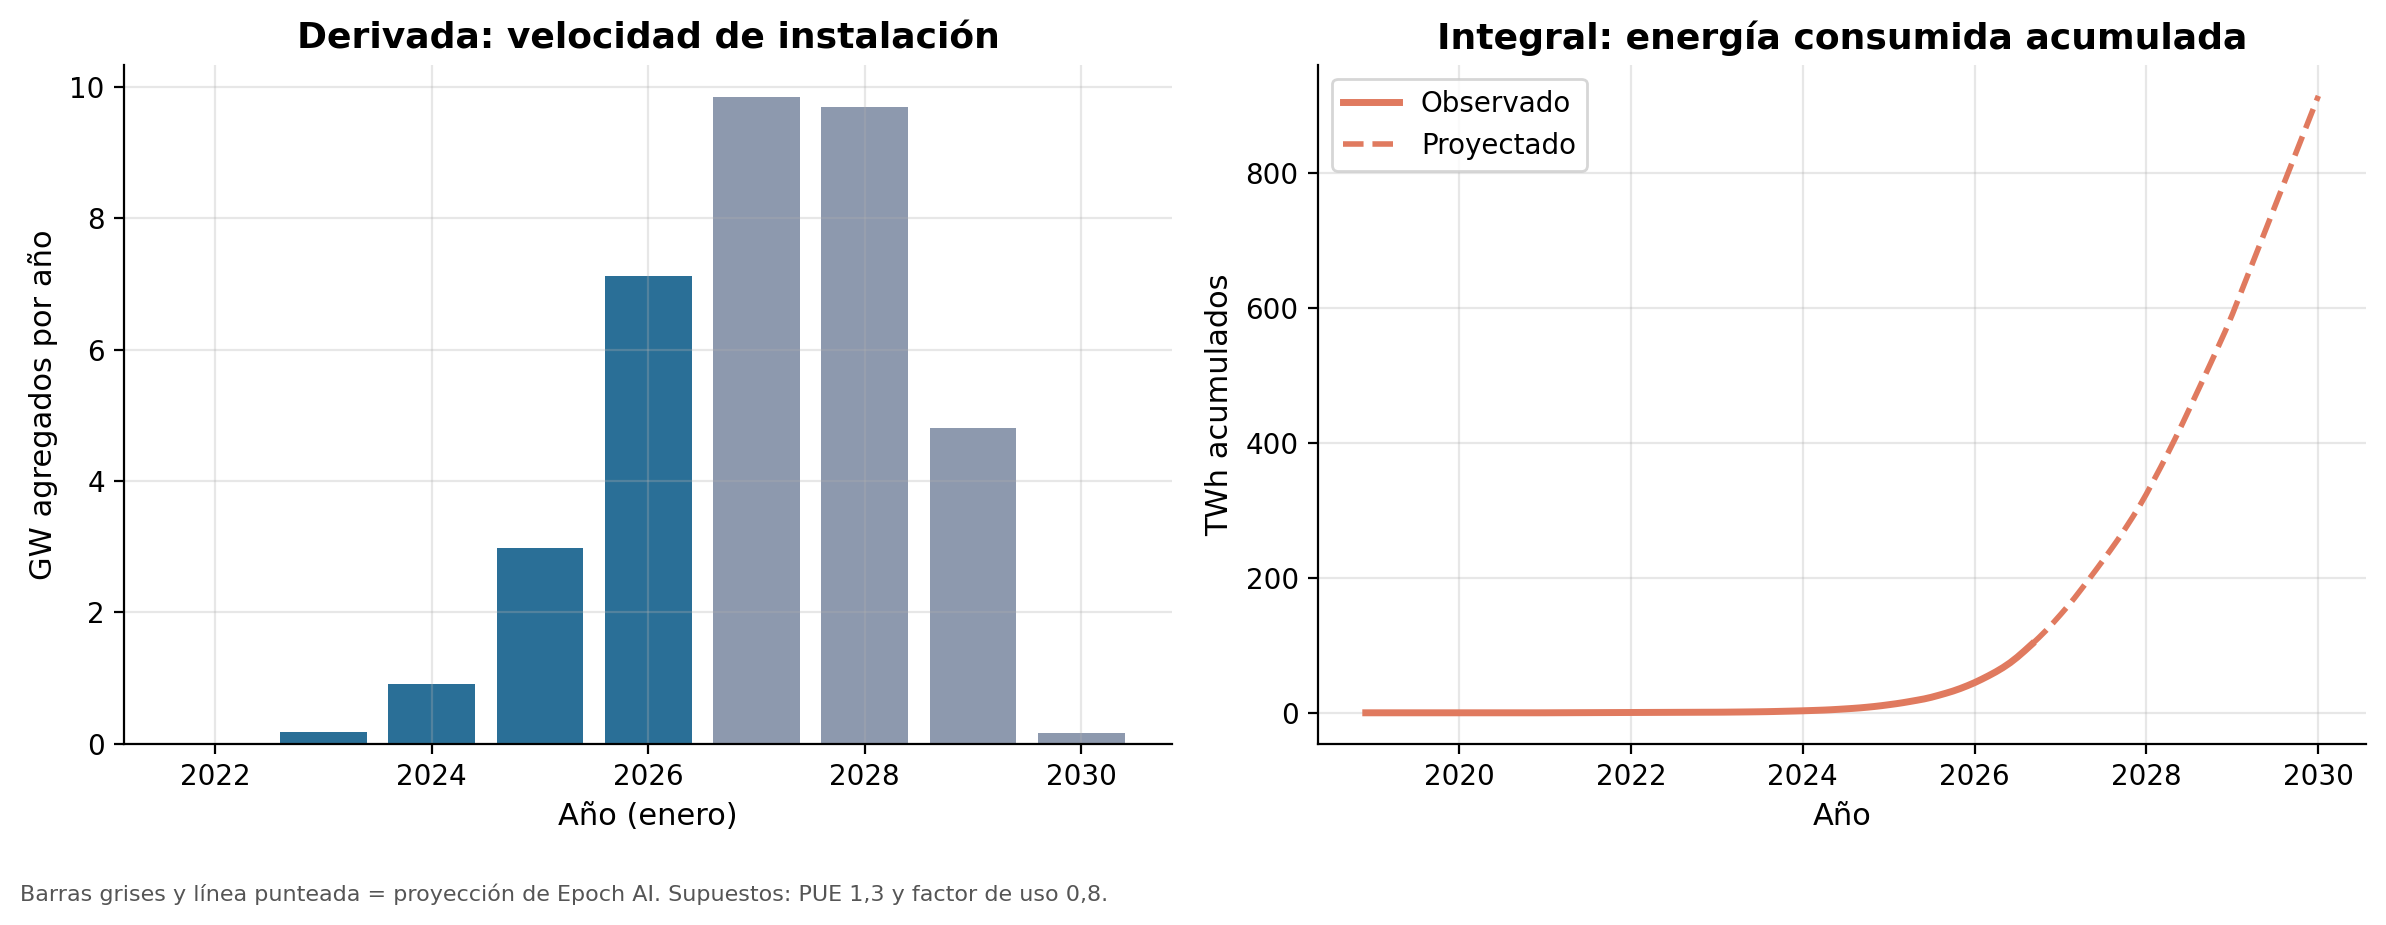
\includegraphics[width=\linewidth]{04_derivada_e_integral.png}
  \caption{Derivada e integral.}
\end{subfigure}
\caption{Evolución de la potencia instalada (línea punteada y barras grises: proyección de Epoch AI).}
\label{fig:potencia}
\end{figure}

\subsection{Concentración y localización}

Cinco empresas —Google, Meta, Amazon, Microsoft y SpaceXAI— concentran el \textbf{77,3\,\%} de la potencia operativa; Google encabeza con 3,3~GW en 17 instalaciones (Figura~\ref{fig:quienes}a). La eficiencia del hardware también difiere: Google y CoreWeave alojan unos 1.200 H100 equivalentes por MW, frente a unos 750 en Amazon, que usa chips propios. Sobre los dueños identificados, el índice de Herfindahl-Hirschman es de 1.623 y las cuatro mayores empresas reúnen el 72,9\,\%: un mercado moderadamente concentrado, cercano al umbral de alta concentración (1.800) de las guías de fusiones de Estados Unidos de 2023.

En Estados Unidos, el cruce con la EIA muestra que los data centers se ubican en estados con \textbf{electricidad industrial más barata}: el precio ponderado por potencia es 7,35~¢/kWh contra 8,13 del promedio nacional, y la mediana es 7,77 en los 27 estados con data centers operativos frente a 8,72 en el resto. La correlación es negativa pero débil ($r=-0{,}28$), lo que sugiere que otros factores —acceso a la red, suelo, incentivos— también pesan. Esa electricidad barata es mayormente \textbf{fósil}: 62\,\% ponderado por potencia, con Ohio (82\,\%) como el estado de mayor capacidad (Figura~\ref{fig:quienes}b).

\begin{figure}[h]
\centering
\begin{subfigure}{0.45\textwidth}
  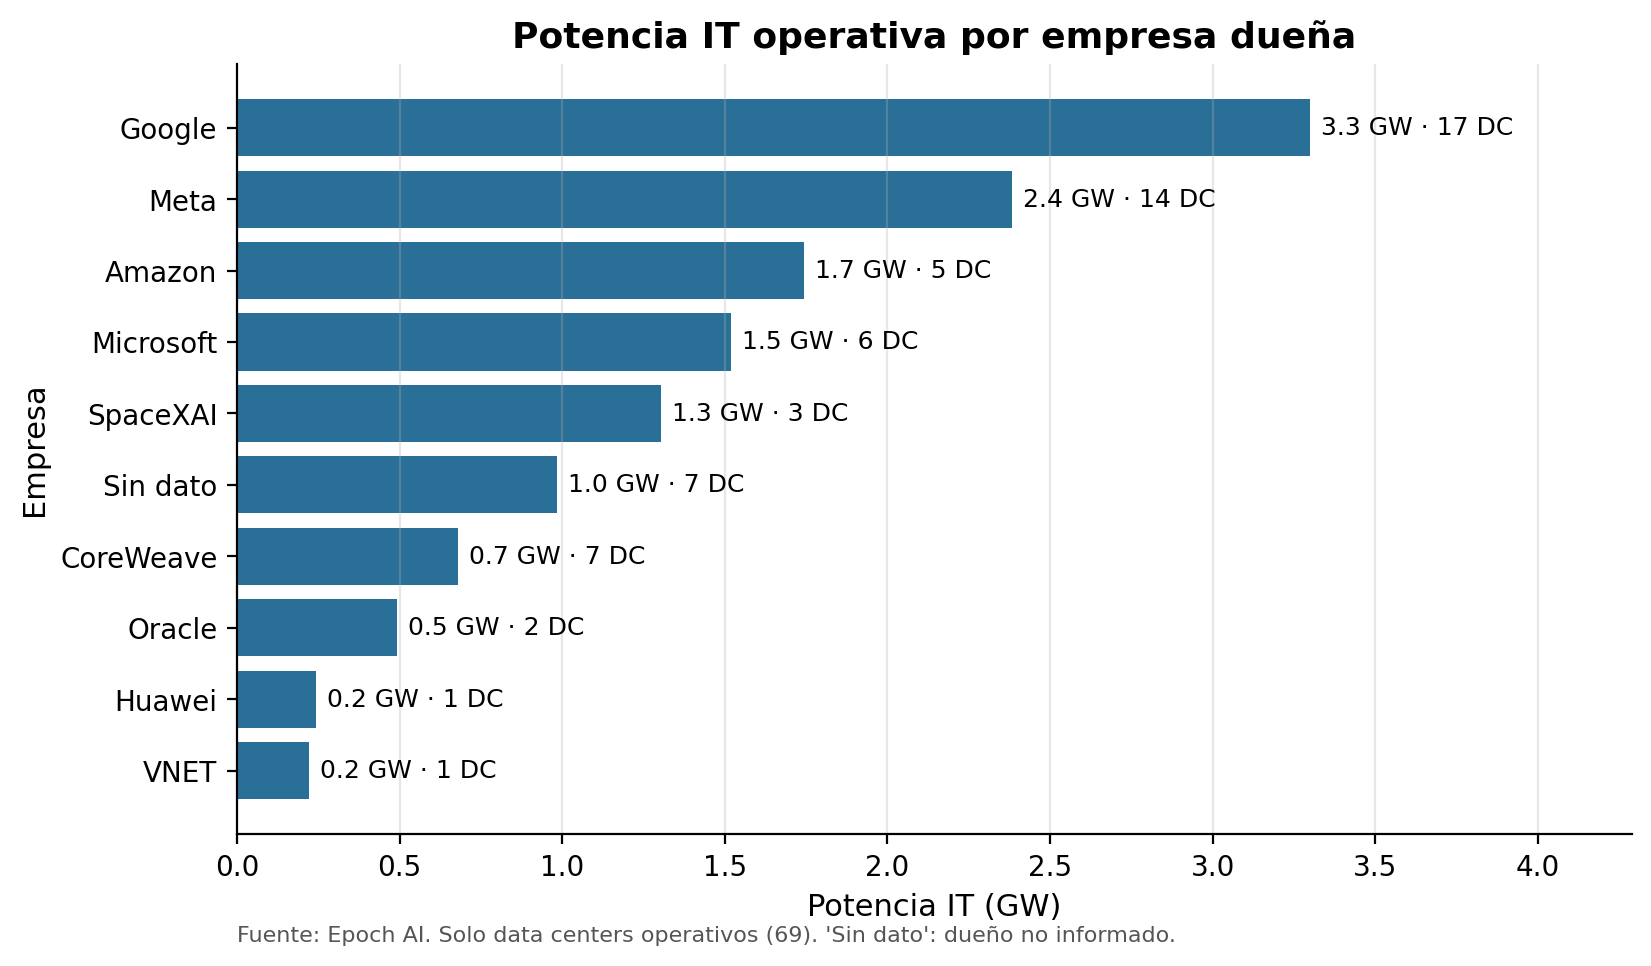
\includegraphics[width=\linewidth]{02_potencia_por_empresa.png}
  \caption{Potencia por empresa.}
\end{subfigure}\hfill
\begin{subfigure}{0.53\textwidth}
  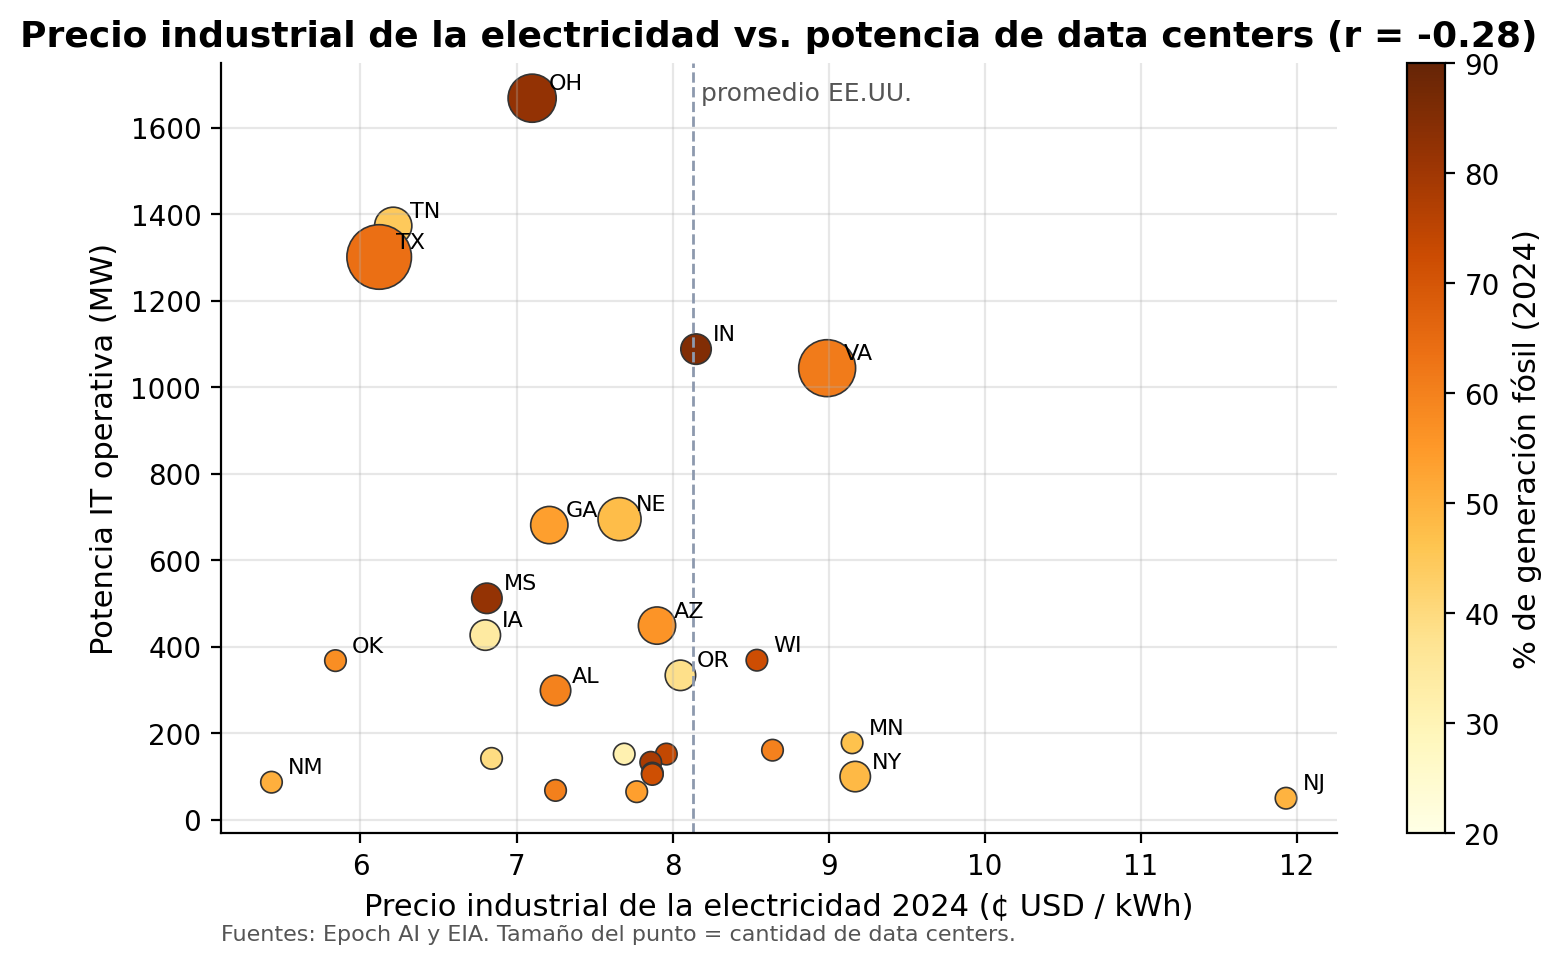
\includegraphics[width=\linewidth]{03_precio_vs_potencia.png}
  \caption{Precio industrial vs. potencia, por estado.}
\end{subfigure}
\caption{Quién controla la potencia y dónde se instala.}
\label{fig:quienes}
\end{figure}

\subsection{Dimensión frente a los países}

Con la potencia actual, el consumo anual estimado es de 118~TWh, el \textbf{73\,\% de la demanda eléctrica argentina} de 2024 (161,7~TWh) y 1,3 veces la de Chile. Con la potencia proyectada llegaría a 325~TWh, \textbf{dos veces la demanda argentina} (Figura~\ref{fig:escenario}a). Valuada al precio industrial ponderado de los estados donde se ubican (73,5~USD/MWh), esa energía implica un gasto de \textbf{USD~8.700 millones anuales}, y de USD~23.900 millones con la potencia proyectada. La conclusión resiste el supuesto de uso: con $u=0{,}6$ el consumo equivale al 55\,\% de la demanda argentina y con $u=1$, al 91\,\%.

Fuera de Estados Unidos el cómputo de IA es escaso. La base de clusters atribuye a ese país el 75,6\,\% de la potencia registrada; en América Latina solo figuran nueve clusters en Brasil —casi todos supercomputadoras de Petrobras de menos de 2~MW— y uno en México. Según la IEA, los data centers usan el 4,9\,\% de la electricidad de Estados Unidos (2025), pero apenas el 0,12\,\% en Centro y Sudamérica, sin cambios desde 2020.

\subsection{Escenario: \emph{Stargate Argentina}}

Un data center de 500~MW operando con PUE~1,3 y uso de 0,8 demandaría \textbf{4,55~TWh anuales, el 2,8\,\% de la demanda eléctrica del país}. Con los coeficientes de Epoch, su costo de capital sería de unos USD~18.900 millones, más USD~450 millones anuales de operación (USD~23.500 millones a diez años), del mismo orden que los USD~25.000 millones anunciados. Al costo monómico proyectado para grandes usuarios en 2026 (67~USD/MWh \cite{aleph}), la electricidad costaría unos \textbf{USD~305 millones por año}, cerca de dos tercios del costo operativo que asigna Epoch.

Las emisiones dependen críticamente de la red que lo abastezca (Tabla~\ref{tab:emisiones} y Figura~\ref{fig:escenario}b): con la intensidad promedio argentina serían 1,57~Mt de CO$_2$ por año, similar a Estados Unidos y once veces más que en Noruega.

\begin{table}[h]
\centering\small
\begin{tabular}{@{}lrrrrrrrr@{}}
\toprule
 & Noruega & Uruguay & Brasil & Canadá & Chile & \textbf{Argentina} & EE.UU. & China \\
\midrule
gCO$_2$/kWh (2024) & 30 & 70 & 106 & 185 & 260 & \textbf{345} & 384 & 555 \\
Mt CO$_2$/año & 0,14 & 0,32 & 0,48 & 0,84 & 1,18 & \textbf{1,57} & 1,75 & 2,53 \\
\bottomrule
\end{tabular}
\caption{Emisiones anuales de un data center de 500~MW según la red eléctrica del país.}
\label{tab:emisiones}
\end{table}

\begin{figure}[h]
\centering
\begin{subfigure}{0.49\textwidth}
  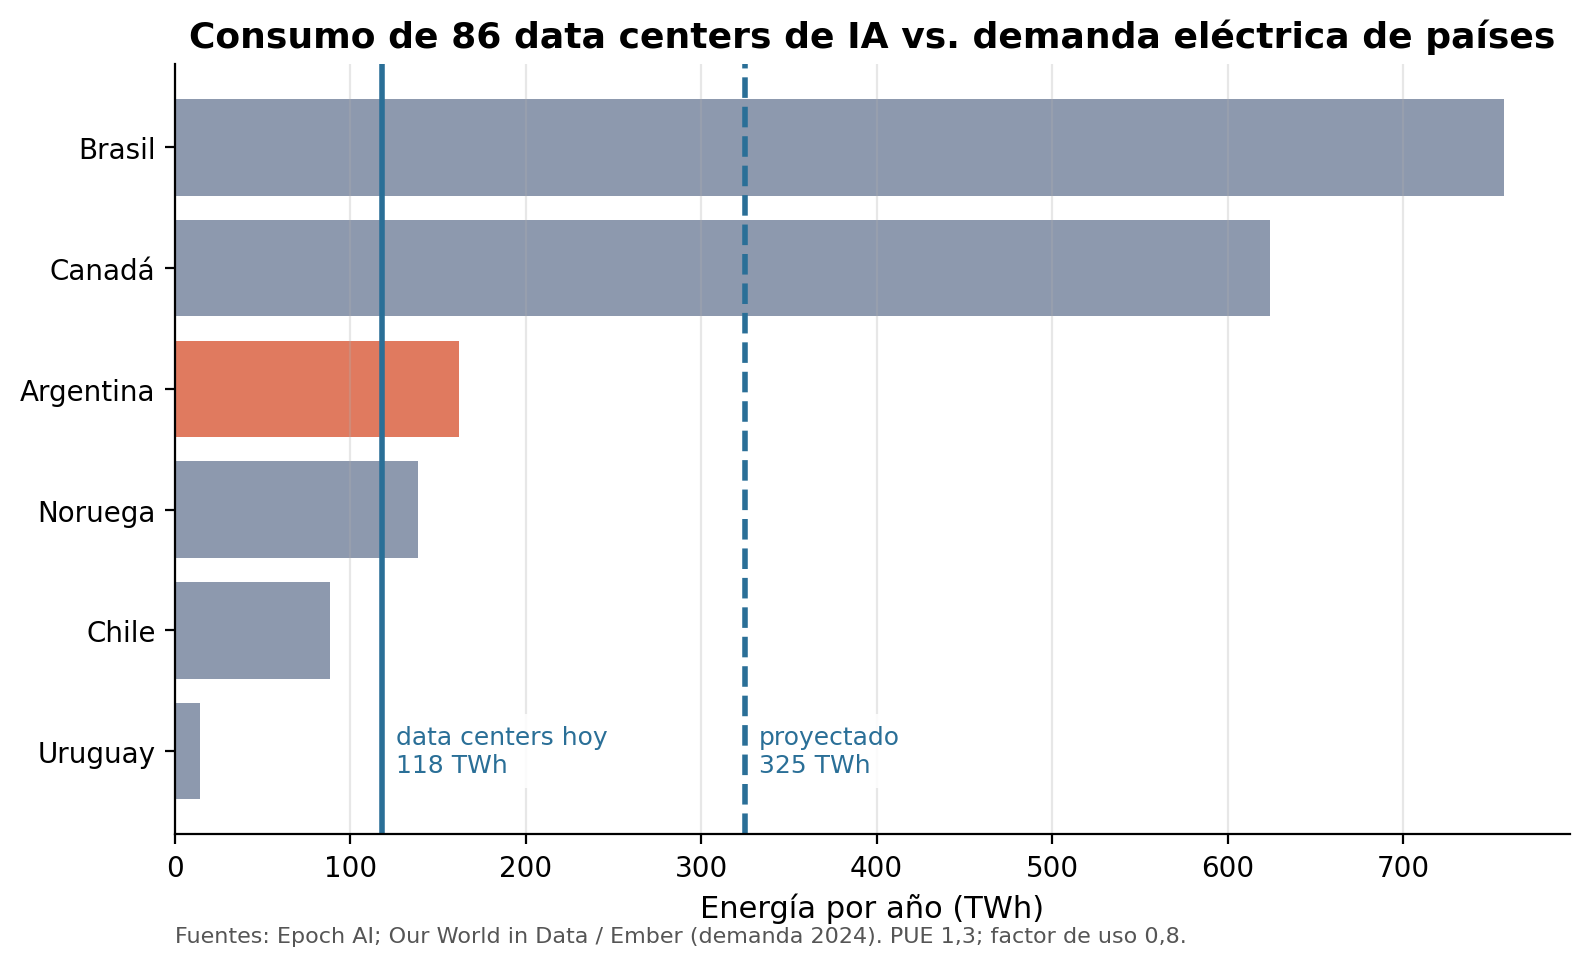
\includegraphics[width=\linewidth]{05_datacenters_vs_paises.png}
  \caption{Consumo vs. demanda de países.}
\end{subfigure}\hfill
\begin{subfigure}{0.49\textwidth}
  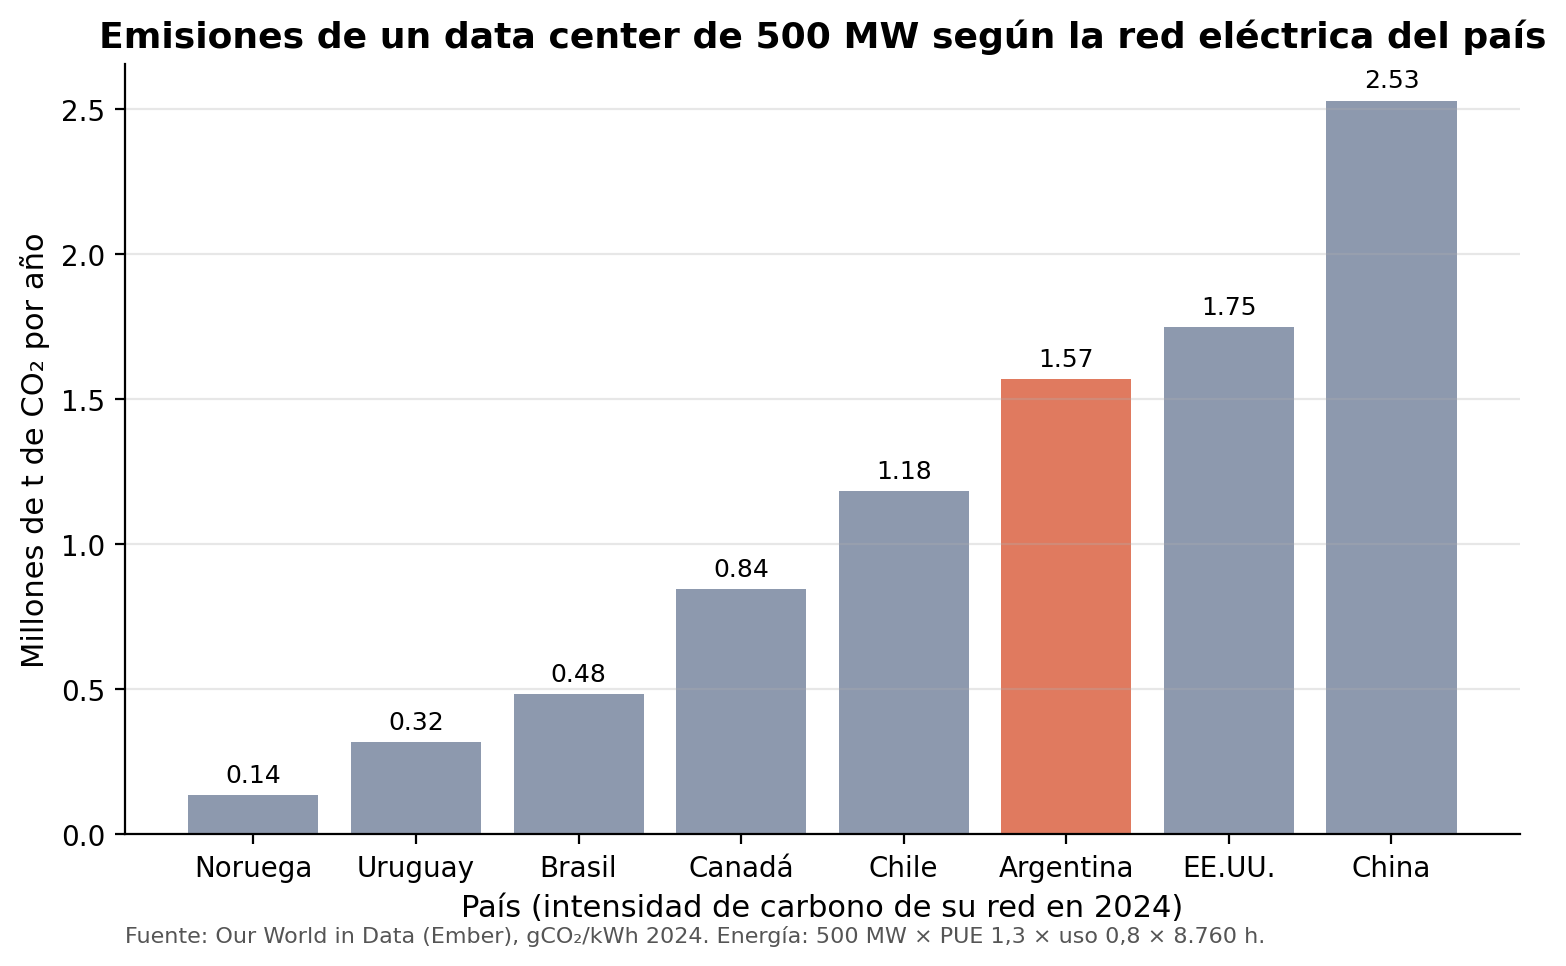
\includegraphics[width=\linewidth]{06_emisiones_escenario_500mw.png}
  \caption{Emisiones de un proyecto de 500~MW.}
\end{subfigure}
\caption{Dimensión energética y ambiental.}
\label{fig:escenario}
\end{figure}

% ═════════════════════════════════════════════════════════════════════════════
\subsection{Extensión: una regresión y un modelo de aprendizaje automático}

\paragraph{Regresión.} Sobre 404 clusters de GPU (2017--2025) se estimó por MCO, con errores robustos, $\ln(\text{kW por H100e}) = a + b\,t + \varepsilon$. La pendiente es $b=-0{,}369$: la potencia necesaria por unidad de cómputo \textbf{cae un 30,9\,\% por año} (IC~95\,\%: $-32{,}4$\,\% a $-29{,}3$\,\%; $R^2=0{,}73$; Figura~\ref{fig:modelos}a). Aun así la demanda total crece, porque el cómputo instalado aumenta mucho más rápido que la eficiencia (paradoja de Jevons). Como Epoch estima parte de la potencia a partir de las especificaciones de los chips, la tendencia refleja sobre todo el recambio de generaciones de hardware.

\paragraph{Aprendizaje automático.} Con una regresión lineal de \texttt{scikit-learn} se predijo el cómputo (H100e) de cada data center a partir de su potencia, entrenando con el 70\,\% de los 69 operativos y evaluando con el 30\,\% restante. El modelo aprende unos 940 H100e por MW, obtiene $R^2=0{,}86$ en los datos de prueba y un error absoluto medio 59\,\% menor que el de un modelo que predice siempre el promedio. Sin embargo, al repetir el sorteo 20 veces el $R^2$ oscila entre 0,20 y 0,95; la validación cruzada de 5 pliegues da $0{,}75 \pm 0{,}15$, y agregar el año de inicio no mejora la predicción (Figura~\ref{fig:modelos}b). Con pocos datos, una única partición puede ser engañosa.

\begin{figure}[h]
\centering
\begin{subfigure}{0.40\textwidth}
  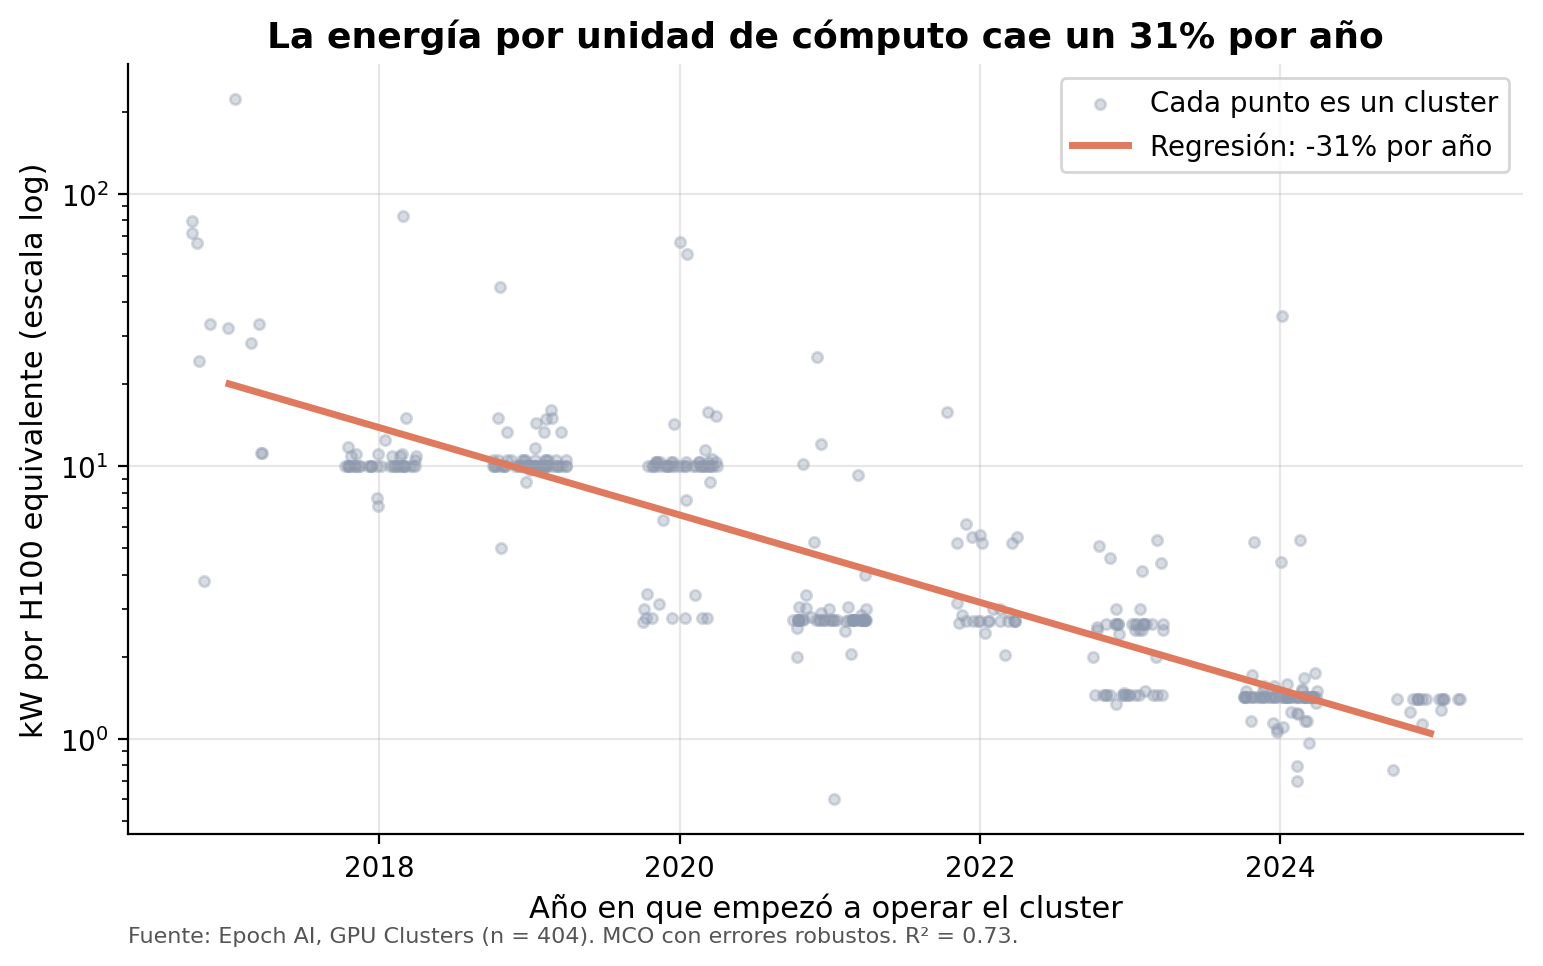
\includegraphics[width=\linewidth]{07_regresion_eficiencia.png}
  \caption{Regresión de eficiencia.}
\end{subfigure}\hfill
\begin{subfigure}{0.58\textwidth}
  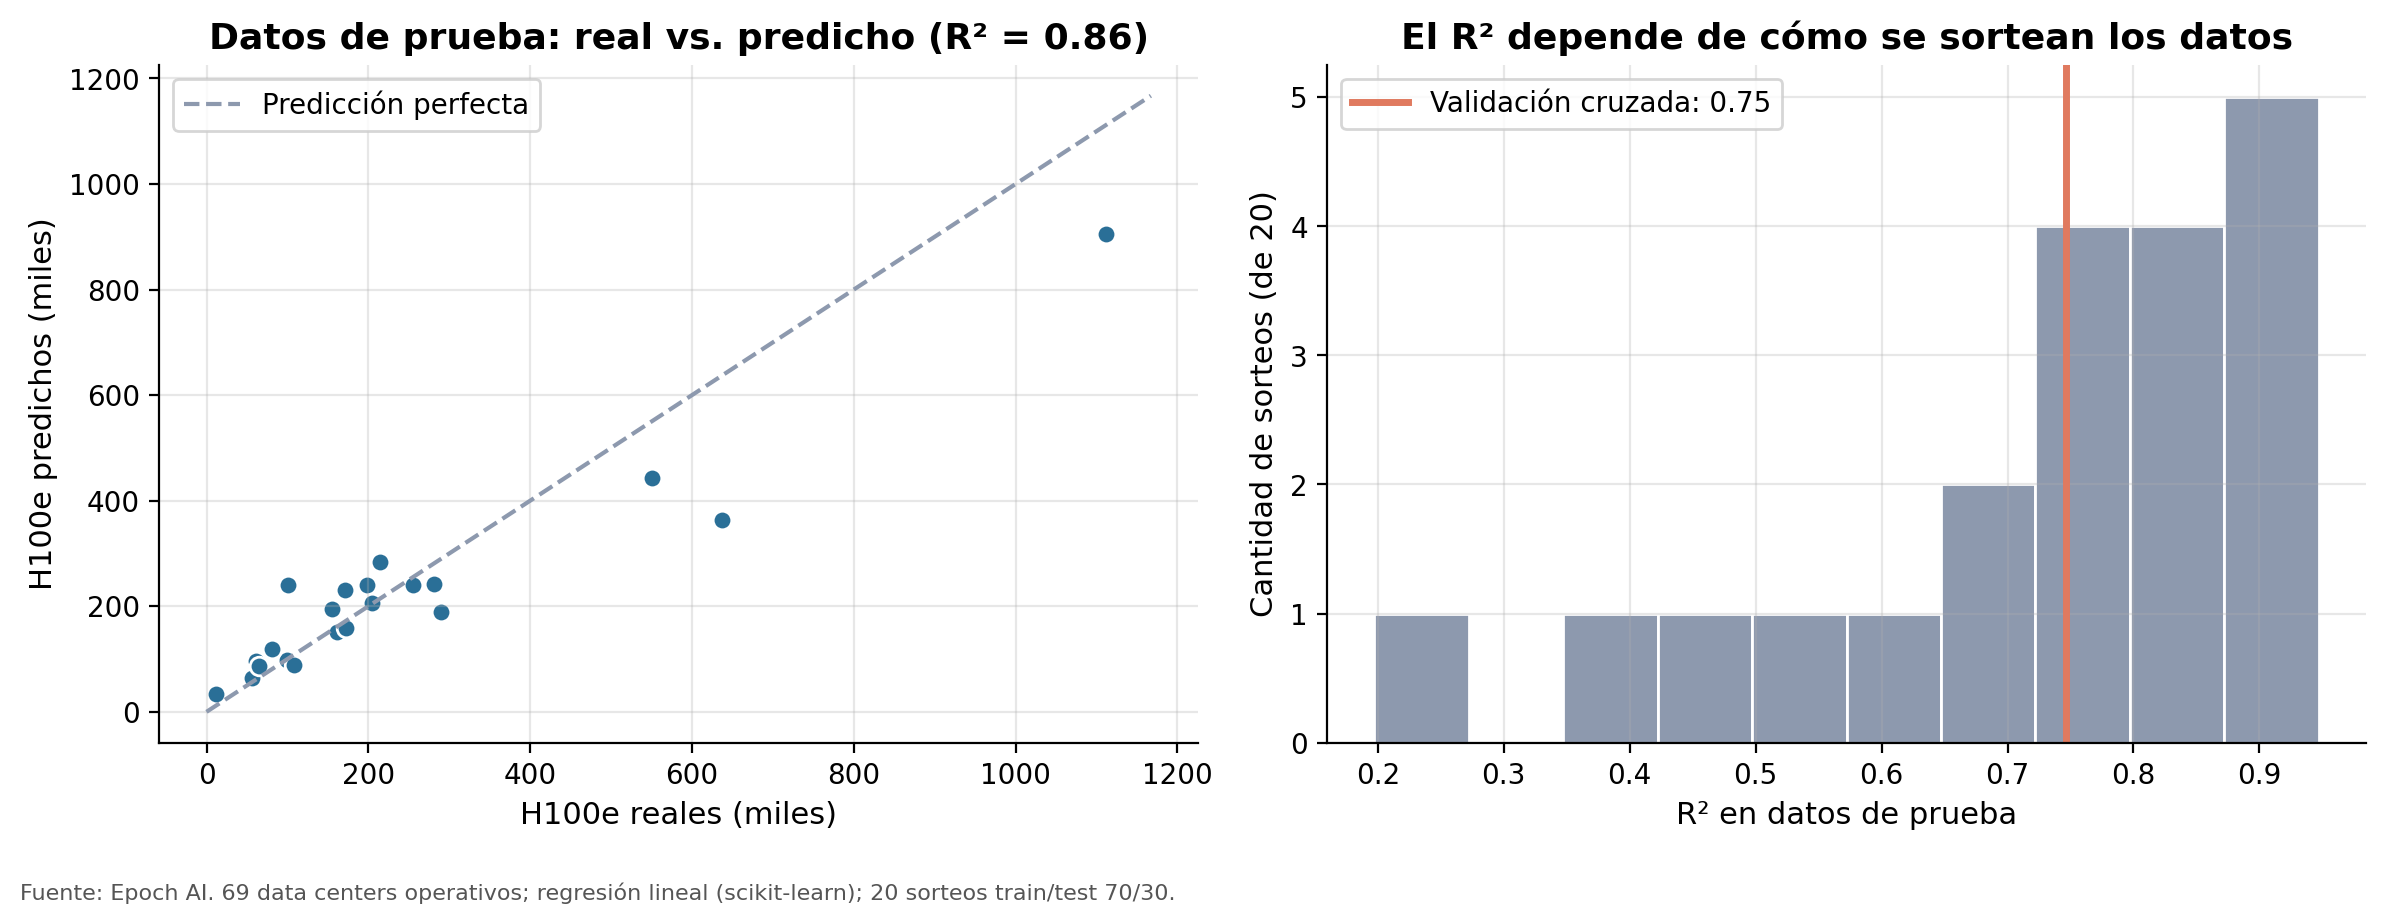
\includegraphics[width=\linewidth]{08_machine_learning.png}
  \caption{Predicción y estabilidad del $R^2$.}
\end{subfigure}
\caption{Modelos: explicar (regresión) y predecir (aprendizaje automático).}
\label{fig:modelos}
\end{figure}

\subsection{Organización industrial: estructura, conducta y desempeño}

\paragraph{Estructura.} La concentración difiere por eslabón (Tabla~\ref{tab:oi}). El más concentrado es el de \textbf{chips}: NVIDIA diseña el 65,6\,\% del cómputo instalado en los data centers relevados y el HHI (4.890) equivale a un mercado de dos empresas iguales. Google (100\,\% de chips propios) y Amazon (91\,\%) están integradas verticalmente, mientras que Meta, Microsoft, SpaceXAI, CoreWeave y Oracle dependen por completo de NVIDIA. La barrera de entrada es del orden de USD~38.000 millones por GW de capacidad.

\paragraph{Conducta.} La industria compite en capacidad. Entre septiembre de 2025 y septiembre de 2026 la energía por unidad de cómputo cayó 23\,\%, pero el cómputo instalado se multiplicó por 4,1 y el gasto eléctrico por 3,1 (de USD~2.760 a 8.660 millones anuales): una \textbf{paradoja de Jevons}. Las salidas a bolsa de Anthropic y OpenAI se inscriben en esa carrera: valuaciones cercanas al billón de dólares exigen prometer crecimiento, que se traduce en cómputo y electricidad pagados antes que los ingresos, en empresas que todavía pierden dinero \cite{fortuneap}. Bain \& Company estima que la industria necesitaría USD~2 billones de ingresos anuales para recuperar la inversión \cite{wm}.

\paragraph{Desempeño.} El índice de Lerner, $L=(P-CMg)/P$, se estimó para el alquiler de GPU con precios de USD~1,49 a 6,98 por hora de H100 \cite{intuition} y costos construidos con los datos del trabajo. El costo marginal de corto plazo (operación, incluida la electricidad) es de USD~0,13 por hora, lo que da $L$ entre 0,92 y 0,98; pero ese valor sobrestima el poder de mercado en una industria con costos fijos enormes. Sumando el capital amortizado en cinco años (USD~1,17 por hora), $L$ cae a un rango de 0,21 a 0,83 según el proveedor. En el eslabón de chips, el margen bruto de NVIDIA (75\,\% en el trimestre a julio de 2026 \cite{nvidia}) aproxima un Lerner elevado, coherente con su participación dominante.

\begin{table}[h]
\centering\small
\begin{tabular}{@{}lccc@{}}
\toprule
 & \textbf{Chips} & \textbf{Data centers} & \textbf{Laboratorios}$^{*}$ \\
\midrule
HHI & 4.890 & 1.623 & 1.934 \\
Líder (participación) & NVIDIA (65,6\,\%) & Google (26,9\,\%) & OpenAI (29,0\,\%) \\
Empresas equivalentes & 2,0 & 6,2 & 5,2 \\
Lerner (aprox.) & $\approx 0{,}75$ & 0,21--0,83 & pérdidas \\
\bottomrule
\end{tabular}
\caption{Estructura y desempeño por eslabón. $^{*}$Medida aproximada: data centers en los que cada laboratorio figura como usuario.}
\label{tab:oi}
\end{table}

% ═════════════════════════════════════════════════════════════════════════════
\section{Conclusiones}

Los grandes data centers de IA ya consumen una cantidad de electricidad comparable a la de un país mediano y su expansión se acelera: el desafío para las redes es la \textbf{velocidad}, no solo el volumen. En Estados Unidos, la búsqueda de electricidad barata los lleva a estados con generación mayormente fósil. Para Argentina, un proyecto de 500~MW sería absorbible en términos de demanda (2,8\,\%) siempre que se acompañe de generación nueva, y su huella de carbono dependería de abastecerse con renovables dedicadas —el argumento eólico de la Patagonia— antes que con la red promedio.

\paragraph{Limitaciones.} (i) Epoch estima potencia, cómputo y costo con intervalos del 80\,\% de $\pm1{,}4\times$ a $\pm1{,}6\times$ y cubre cerca del 46\,\% de la capacidad mundial; (ii) el costo es un coeficiente fijo, útil para escenarios pero no para medir economías de escala; (iii) el factor de uso es un supuesto; (iv) la intensidad de carbono es el promedio de la red, no el contrato específico de cada instalación; (v) \emph{Stargate Argentina} es aún una carta de intención.

\paragraph{Extensiones.} Incorporar precios mayoristas de CAMMESA para estimar el costo energético en Argentina; analizar el uso de agua cuando mejore su cobertura; estimar economías de escala con los costos de hardware de la base de clusters, controlando por generación del chip.

% ═════════════════════════════════════════════════════════════════════════════
\section{Reflexión metodológica}

El trabajo se realizó con asistencia de un modelo de lenguaje (Claude) en código, verificación de unidades y borradores de texto; las celdas asistidas y sus \emph{prompts} están indicadas en el notebook. La revisión humana fue decisiva en tres puntos: (1) detectar que el costo de Epoch era un coeficiente fijo, lo que obligó a reemplazar la aplicación prevista (funciones de costo) por derivadas e integrales; (2) contrastar cada afirmación con las salidas del notebook, lo que corrigió cifras del primer borrador (una tasa de instalación sobreestimada y una participación de Estados Unidos redondeada al alza) y eliminó un dato sin fuente; y (3) validar los cruces reescribiéndolos en SQL. El aprendizaje central es que \textbf{antes de modelar hay que entender cómo se construyó cada variable y verificar qué claves se pierden al unir tablas}.

% ── Referencias ──────────────────────────────────────────────────────────────
\begin{thebibliography}{9}\small
\bibitem{epochdc} Epoch AI (2026). \emph{AI Data Centers}. \url{https://epoch.ai/data/ai-data-centers}
\bibitem{epochgpu} Epoch AI (2026). \emph{GPU Clusters}. \url{https://epoch.ai/data/gpu-clusters}
\bibitem{eia} U.S. Energy Information Administration (2025). \emph{State Electricity Data}. \url{https://www.eia.gov/electricity/data/state/}
\bibitem{owid} Our World in Data (2026). \emph{Energy}; datos de Ember e IEA. \url{https://ourworldindata.org/energy}
\bibitem{iea} International Energy Agency (2025). \emph{Energy and AI}. \url{https://www.iea.org/reports/energy-and-ai}
\bibitem{dcd} DatacenterDynamics (2025). \emph{OpenAI plans 500MW data center in Argentina}. \url{https://www.datacenterdynamics.com/en/news/openai-plans-500mw-data-center-in-argentina/}
\bibitem{aleph} Aleph Energy (2026). Proyecciones de precios del MEM para 2026 con datos de CAMMESA, citado en \emph{Mejor Energía}, 21 de enero de 2026.
\bibitem{cnbcanthropic} CNBC (2026). \emph{Anthropic confidentially files IPO prospectus with SEC}, 1 de junio de 2026.
\bibitem{tcopenai} TechCrunch (2026). \emph{OpenAI files confidentially for IPO, following Anthropic}, 8 de junio de 2026.
\bibitem{fortuneap} Fortune / Associated Press (2026). \emph{Anthropic IPO filing and AI bubble comparisons}, 2 de junio de 2026.
\bibitem{wm} Washington Monthly (2026). \emph{An AI Crash Is Coming. What Then?}, 3 de mayo de 2026.
\bibitem{intuition} IntuitionLabs (2026). \emph{H100 Rental Prices Compared Across Cloud Providers}, actualizado el 16 de agosto de 2026.
\bibitem{nvidia} NVIDIA (2026). \emph{Financial Results for Second Quarter Fiscal 2027}, 26 de agosto de 2026.
\end{thebibliography}

% ═════════════════════════════════════════════════════════════════════════════
\appendix
\section{Diccionario de variables}

\begin{table}[h]
\centering\small
\begin{tabularx}{\textwidth}{@{}l l X@{}}
\toprule
\textbf{Variable} & \textbf{Fuente} & \textbf{Descripción} \\
\midrule
\texttt{mw\_it} & Epoch & Potencia de los servidores (MW), sin refrigeración \\
\texttt{mw\_total} & Epoch & Potencia total de la instalación (MW) \\
\texttt{h100e} & Epoch & Cómputo expresado en chips NVIDIA H100 equivalentes \\
\texttt{capex\_usd\_bn} & Epoch & Costo de capital estimado (miles de millones de USD de 2025) \\
\texttt{duenio} & Epoch & Empresa dueña, sin etiqueta de confianza \\
\texttt{estado} & derivada & Estado de EE.UU. extraído de la dirección \\
\texttt{operativo} & derivada & Verdadero si \texttt{mw\_it} $>0$ \\
\texttt{h100e\_por\_mw} & derivada & Cómputo por MW (eficiencia del hardware) \\
\texttt{precio\_industrial} & EIA & Precio medio industrial de la electricidad (¢ USD/kWh) \\
\texttt{pct\_fosil} & EIA (derivada) & \% de la generación del estado a carbón, gas y petróleo \\
\texttt{gco2\_kwh} & OWID & Intensidad de carbono de la red del país \\
\texttt{demanda\_twh} & OWID & Demanda eléctrica total del país (TWh) \\
\bottomrule
\end{tabularx}
\end{table}

\section{Consultas SQL de validación}

\begin{lstlisting}
-- Clusters de GPU + intensidad de carbono + demanda, por pais
SELECT c.pais, COUNT(*) AS clusters, SUM(c.mw) AS mw,
       i.gco2_kwh, dm.demanda_twh
FROM clusters c
LEFT JOIN intensidad_2024 i  ON c.pais = i.pais
LEFT JOIN demanda_2024    dm ON c.pais = dm.pais
WHERE c.pais IS NOT NULL
GROUP BY c.pais
ORDER BY mw DESC;

-- Anti-join: paises de los clusters sin intensidad de carbono
SELECT DISTINCT c.pais
FROM clusters c
LEFT JOIN intensidad_2024 i ON c.pais = i.pais
WHERE i.pais IS NULL AND c.pais IS NOT NULL;

-- Todos los hitos de obra tienen su data center?
SELECT COUNT(DISTINCT t.nombre) AS data_centers_en_timeline,
       COUNT(DISTINCT CASE WHEN d.nombre IS NULL THEN t.nombre END) AS sin_pareja
FROM timelines t
LEFT JOIN data_centers d ON t.nombre = d.nombre;
\end{lstlisting}

\end{document}
